% Created 2017-04-26 三 01:30
\documentclass[11pt]{article}
\usepackage[utf8]{inputenc}
\usepackage[T1]{fontenc}
\usepackage{fixltx2e}
\usepackage{graphicx}
\usepackage{longtable}
\usepackage{float}
\usepackage{wrapfig}
\usepackage{rotating}
\usepackage[normalem]{ulem}
\usepackage{amsmath}
\usepackage{textcomp}
\usepackage{marvosym}
\usepackage{wasysym}
\usepackage{amssymb}
\usepackage{hyperref}
\tolerance=1000
\author{Qiu Wei}
\date{\today}
\title{MPML REPORT}
\hypersetup{
  pdfkeywords={},
  pdfsubject={},
  pdfcreator={Emacs 24.5.1 (Org mode 8.2.10)}}
\begin{document}

\maketitle
\tableofcontents

\begin{abstract}
This document describes the experiment result of python ver.
Data analysis will be added soon.
\end{abstract}

\section{Trainning Result}
\label{sec-1}
The trainning result is as following:
\begin{center}
\begin{tabular}{rllrlrr}
\hline
No. & Algorithm & ? & Time/s & Accuracy & F1 value & AUC value\\
\hline
1 & brute svm & $\backslash$ & 34.04 & 96.37167\% & 0.92404 & 0.48782\\
2 & random min-max & serialized & 305.47 & 96.26846\% & 0.92194 & $\backslash$\\
3 & random min-max & parallelized & 140.08 & 96.26846\% & 0.92184 & 0.48307\\
4 & labeled min-max & serialized & 204.35 & 96.71042\% & 0.93101 & $\backslash$\\
5 & labeled min-max & parallelized & 204.35 & 96.69719\% & 0.93074 & 0.48567\\
\hline
\end{tabular}
\end{center}
The random min-max algorithm separate the input data into 5 parts randomly(5*5 models).
The labeled min-max seperate the input data via the first two letters(4*12 models).

The total contains the time of load data, save model and other IO operations.
Parsing is finished before the program runs.

The ROC Graph is as following:


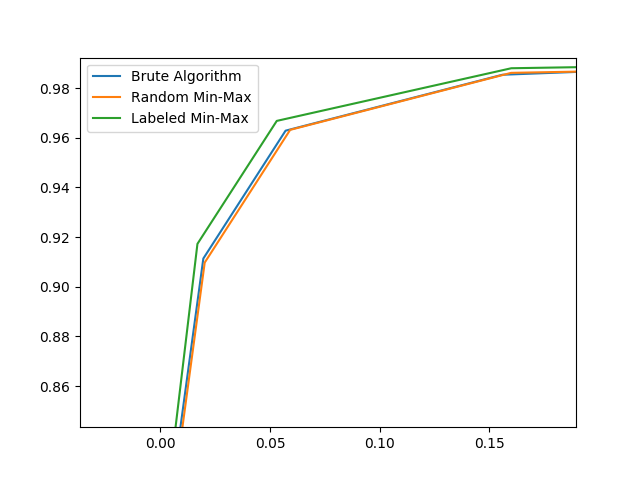
\includegraphics[width=.9\linewidth]{figure_1.png}



The time cost between serialized min-max and parallelized min-max is:

\begin{center}
\begin{tabular}{rllrrr}
\hline
No. & Parallelized? & Algorithm & Trainning time/s & Testing time/s & Total time/s\\
\hline
1 & Yes & labeled & 59.37346 & 144.54046 & 203.93383\\
2 & No & labeled & 115.96271 & 371.83840 & 489.00508\\
3 & Yes & random & 54.49303 & 84.16756 & 138.69087\\
4 & No & random & 103.98813 & 200.19163 & 305.47026\\
\hline
\end{tabular}
\end{center}


Test environment is Ubuntu, 4 kernal.
Python version is 3.5.
% Emacs 24.5.1 (Org mode 8.2.10)
\end{document}